\documentclass[xcolor=pdftex,dvipsnames]{beamer}
\usepackage{beamerthemesplit,hyperref}
\usetheme{default}
\usecolortheme{dove}
%\setbeamertemplate{background}[grid][step=1cm]
\setbeamertemplate{caption}{\raggedright\insertcaption\par}
\usepackage[absolute,overlay]{textpos}
\usepackage{graphicx}


\usepackage{listings,multirow,amssymb,amsmath,cancel,float,color}
\usepackage{pgfpages}
%\usepackage{listings}
%\lstset{language=Python,
%    basicstyle=\ttfamily\bfseries,
%    commentstyle=\color{red}\itshape,
%    stringstyle=\color{darkgreen},
%    showstringspaces=false,
%    keywordstyle=\color{blue}\bfseries}

\usepackage{fontspec}
\usepackage{minted}
\usepackage{tcolorbox}
\usepackage{etoolbox}
\BeforeBeginEnvironment{minted}{\begin{tcolorbox}}%
\AfterEndEnvironment{minted}{\end{tcolorbox}}%

%\setsansfont{Calibri}
%\setmonofont{Consolas}

%\renewcommand{\theFancyVerbLine}{
%  \sffamily\textcolor[rgb]{0.5,0.5,0.5}{\scriptsize\arabic{FancyVerbLine}}}


\graphicspath{{figures/}}

%\setbeamertemplate{navigation symbols}{} 
%\setbeamertemplate{footline}[text line]{SUSY on the Lattice}

\mode<presentation>
\title[]{Cython for HPC}
\author[]{Niall Moran}
\date{July, 2016}
%\titlegraphic{\includegraphics[width=2.5cm]{NUIM-Logo-Main.pdf}}
\setbeamerfont{citation_font}{size=\tiny}
\setbeamerfont{smallerfont}{size=\small}

%\setbeameroption{show notes on second screen}
%\setbeameroption{show notes}
%\xdefinecolor{abricot}{named}{Apricot}

\newcommand{\ua}{\uparrow}
\newcommand{\da}{\downarrow}
\newcommand{\dg}{\dagger}
\newcommand{\nin}{\noindent}
\newcommand{\non}{\nonumber}
\newcommand{\pd}{\partial}
\newcommand{\bea}{\begin{eqnarray}}
\newcommand{\eea}{\end{eqnarray}}
\newcommand{\be}{\begin{equation}}
\newcommand{\ee}{\end{equation}}
\newcommand{\ba}{\begin{align}}
\newcommand{\ea}{\end{align}}
\newcommand{\braket}[2]{\langle #1|#2\rangle}
\newcommand{\ket}[1]{     |    \,    #1    \rangle}
\newcommand{\bra}[1]{  \langle #1  \,  |} 
\newcommand{\ZZ}{\mathbb{Z}}
\newcommand{\rmi}{\mathrm{i}}
\newcommand{\q}{{\bf q}}
\newcommand{\anb}{b^{\phantom\dagger}}
\newcommand{\crb}{b^\dagger}
\newcommand{\anc}{c^{\phantom\dagger}}
\newcommand{\crc}{c^\dagger}
\newcommand{\bi}{{\boldsymbol{i}}}
\newcommand{\bj}{{\boldsymbol{j}}}
\newcommand{\bk}{{\boldsymbol{k}}}
\newcommand{\bl}{{\boldsymbol{l}}}
\newcommand{\bx}{{\boldsymbol{x}}}
\newcommand{\bq}{{\boldsymbol{q}}}
\newcommand{\bp}{{\boldsymbol{p}}}
\newcommand{\bn}{{\boldsymbol{n}}}
\newcommand{\bs}[1]{ \boldsymbol{#1} }
\newcommand{\abs}[1]{|#1|}


\begin{document}


\begin{frame}\titlepage
\end{frame}


\begin{frame}
	\frametitle{Overview}
	\begin{itemize}
		\item Motivation
		\item Why (not) Python?
		\item Cython
		\item Examples
	\end{itemize}
	\note{Overview slide}
\end{frame}

\begin{frame}[t]
	  \frametitle{Hall Effect}
    \begin{textblock*}{6cm}(1cm,2cm) % {block width} (coords)
    \begin{itemize}
    \item Edwin Hall (1879)
    \item Magnetic field induces Hall current
    \end{itemize}
    \end{textblock*}

    \begin{textblock*}{4cm}(8cm,1.5cm) % {block width} (coords)
    \includegraphics[width=4cm]{HallEffectCartoon}
    \end{textblock*}

    \begin{textblock*}{6cm}(1cm,6cm) % {block width} (coords)
    \includegraphics[width=6cm]{FQHE_diagram}
    \end{textblock*}

    \begin{textblock*}{3cm}(8cm,6cm) % {block width} (coords)
    \visible<2->{\includegraphics[width=3cm]{joystick}}
    \end{textblock*}

\end{frame}
    
\begin{frame}[t]
	  \frametitle{(Integer) Quantum Hall Effect}
    \begin{textblock*}{6cm}(1cm,2cm) % {block width} (coords)
    \begin{itemize}
    \item von Klitzing (1980)
    \item Lower temperature, plateaus appear
    \item Quantization of conductance 
    \end{itemize}
    \end{textblock*}

    \begin{textblock*}{4cm}(8cm,1.5cm) % {block width} (coords)
    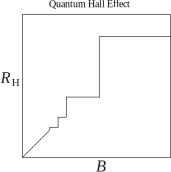
\includegraphics[width=4cm]{QuantumHallEffectCartoon}
    \end{textblock*}

    \begin{textblock*}{6cm}(1cm,6cm) % {block width} (coords)
    \includegraphics[width=6cm]{FQHE_diagram}
    \end{textblock*}

    \begin{textblock*}{3cm}(8cm,6cm) % {block width} (coords)
    \visible<2->{\includegraphics[width=3cm]{multimetre}}
    \end{textblock*}

\end{frame}

\begin{frame}[t]
	  \frametitle{Fractional Quantum Hall Effect}
    \begin{textblock*}{6cm}(1cm,2cm) % {block width} (coords)
    \begin{itemize}
    \item Tsui, Stormer and Gossard (1982)
    \item Plateaus at fractional filling
    \item Anyonic excitations
    \end{itemize}
    \end{textblock*}

    \begin{textblock*}{5cm}(7cm,2cm) % {block width} (coords)
    \includegraphics[width=5cm]{FQHE_plateaus}
    \end{textblock*}

    \begin{textblock*}{6cm}(1cm,6cm) % {block width} (coords)
    \includegraphics[width=6cm]{FQHE_diagram}
    \end{textblock*}

    \begin{textblock*}{3cm}(8cm,6cm) % {block width} (coords)
    \visible<2->{\includegraphics[width=3cm]{question-mark-nothing}}
    \end{textblock*}

\end{frame}

\begin{frame}[t]
    \frametitle{Modelling}
    \begin{textblock*}{12cm}(1cm,1.5cm) % {block width} (coords)
    \begin{itemize}
       \item Finite system $N$ particles and $N_{\phi}$ flux with $\nu = \frac{N}{N_{\phi}}$
       \item Decompose into magnetic orbitals
    \end{itemize}
    \end{textblock*}
    \begin{textblock*}{9cm}(2cm,4cm) % {block width} (coords)
        
\includegraphics[width=9cm]{effective_1d_model}
    \end{textblock*}

    \begin{textblock*}{12cm}(1cm,5.5cm) % {block width} (coords)
    Ways to fill available orbitals
    \end{textblock*}
\end{frame}

\begin{frame}[t]
    \frametitle{Modelling}
    \begin{textblock*}{12cm}(1cm,1.5cm) % {block width} (coords)
    \begin{itemize}
       \item Finite system $N$ particles and $N_{\phi}$ flux with $\nu = \frac{N}{N_{\phi}}$
       \item Decompose into magnetic orbitals
    \end{itemize}
    \end{textblock*}
    \begin{textblock*}{9cm}(2cm,4cm) % {block width} (coords)
        
\includegraphics[width=9cm]{effective_1d_model2}
    \end{textblock*}

    \begin{textblock*}{12cm}(1cm,5.5cm) % {block width} (coords)
    Ways to fill available orbitals
    \end{textblock*}
\end{frame}


\begin{frame}[t]
    \frametitle{Modelling}
    \begin{textblock*}{12cm}(1cm,1.5cm) % {block width} (coords)
    \begin{itemize}
       \item Finite system $N$ particles and $N_{\phi}$ flux with $\nu = \frac{N}{N_{\phi}}$
       \item Decompose into magnetic orbitals
    \end{itemize}
    \end{textblock*}
    \begin{textblock*}{9cm}(2cm,4cm) % {block width} (coords)
        \includegraphics[width=9cm]{effective_1d_model3}
    \end{textblock*}

    \begin{textblock*}{12cm}(1cm,5.5cm) % {block width} (coords)
    Ways to fill available orbitals
    \begin{equation*}
      {N_{\phi}\choose N} \approx f(\nu)^N
    \end{equation*}
    \end{textblock*}
\end{frame}

\begin{frame}[t]
    \frametitle{Modelling}
    \begin{textblock*}{12cm}(1cm,1.5cm) % {block width} (coords)
    \begin{itemize}
       \item Finite system $N$ particles and $N_{\phi}$ flux with $\nu = \frac{N}{N_{\phi}}$
       \item Decompose into magnetic orbitals
    \end{itemize}
    \end{textblock*}
    \begin{textblock*}{9cm}(2cm,4cm) % {block width} (coords)
        \includegraphics[width=9cm]{effective_1d_model_superposition}
    \end{textblock*}

    \begin{textblock*}{12cm}(1cm,5.5cm) % {block width} (coords)
    Ways to fill available orbitals
    \begin{equation*}
      {N_{\phi}\choose N} \approx f(\nu)^N
    \end{equation*}
    Wave-function is complex vector of this dimension!
    \end{textblock*}
\end{frame}



\begin{frame}[t]
    \frametitle{Computations}
    \begin{textblock*}{6cm}(0.5cm,3cm) % {block width} (coords)
    \begin{itemize}
       \item Linear algebra 
       \item Markov-Chain Monte Carlo
       \item Tensor network methods
    \end{itemize}
    \end{textblock*}
    \begin{textblock*}{6cm}(7cm,1cm) % {block width} (coords)
      \begin{figure}
        \includegraphics[width=6cm]{N6_2s18_sparsity}
        \caption{6 particles with 18 flux}
      \end{figure}
    \end{textblock*}
\end{frame}


\begin{frame}
  \frametitle{Diminishing returns}
  \begin{columns}
    \begin{column}{6.5cm}
      \begin{center}
        \visible<1->{\begin{figure}
        \includegraphics[width=0.6\linewidth]{laptop}\\
        \caption{10-12 electrons}
        \end{figure}}
      \end{center}
    \end{column}
    \begin{column}{6.5cm}
      \begin{center}
        \visible<2->{\begin{figure}
          \includegraphics[width=.7\linewidth]{supercomputer}\\
        \caption{16-20 electrons}
        \end{figure}}
      \end{center}
    \end{column}
    \begin{column}{6cm}
    \end{column}
  \end{columns}
\end{frame}


\begin{frame}
  \frametitle{Why (not) use Python}
  \visible<1->{Cons
  \begin{itemize}
    \item Slow
    \item GIL
    \item Resource usage
  \end{itemize}}
  \visible<2->{
  Pros
  \begin{itemize}
    \item Fast development, debugging
    \item Amount of packages available
    \item Plotting
    \item Good glue
    \end{itemize}}
\end{frame}


\begin{frame}[t]
    \frametitle{Cython}
    \begin{textblock*}{7cm}(3cm,1cm) % {block width} (coords)
    \includegraphics[width=7cm]{cython_logo}
    \end{textblock*}
    \begin{textblock*}{12cm}(1cm,2cm) % {block width} (coords)
    \begin{itemize}
      \item Superset of python
      \item Compiles to C code
      \item Best of both worlds
      \item Good for wrapping existing C code
    \end{itemize}
    Provides speed increase by
    \begin{itemize}
      \item Compiling
      \item Providing explicit types and functions
      \item Can release the GIL
    \end{itemize}
    \end{textblock*}
\end{frame}


\begin{frame}[fragile]
  \frametitle{Hello World}
  Create hello.pyx containing
  \begin{minted}{python}
print("Hello world!")
  \end{minted}
  and setup.py containing
  \begin{minted}{python}
from distutils.core import setup
from Cython.Build import cythonize

setup(
    ext_modules = cythonize("hello.pyx")
)
  \end{minted}
  then run on command line
  \begin{minted}{bash}
$ python setup.py build_ext --inplace
  \end{minted}

\end{frame}


\begin{frame}[fragile]
  \frametitle{Notebook}
  Load the cython extension

  \begin{minted}{python}
%load_ext Cython
  \end{minted}

  Can now create cython blocks
  \begin{minted}{python}
%%cython
print("Hello world!")
  \end{minted}

  Annotation 
  \begin{minted}{python}
%%cython -a
print("Hello world!")
  \end{minted}
\end{frame}


\begin{frame}[fragile]
  \frametitle{Demonstration}
\begin{minted}{python}
def mean_plain(A, N):
    sum = 0.0
    j = 0
    while j < N:
        sum += A[j]
        j+=1

    return sum / N
\end{minted}
220ms for array of 1\,000\,000 elements
\end{frame}


\begin{frame}[fragile]
  \small
\begin{minted}{python}
cimport numpy as np
cimport cython

@cython.boundscheck(False)
@cython.wraparound(False)
def mean_cython4(
      np.ndarray[np.float64_t, ndim=1, mode="c"] A,
      int N
    ):
    cdef double sum = 0.0
    cdef int j = 0

    while j < N:
        sum += A[j]  
        j += 1

    return sum / N
\end{minted}
1ms for array of 1\,000\,000 elements
\end{frame}


\begin{frame}
  \frametitle{Matrix multiplication benchmark}
  \begin{textblock*}{10cm}(3cm,1cm)
  \includegraphics[width=6cm]{benchmark}
  \end{textblock*}
\end{frame}


\begin{frame}
    \frametitle{Conclusions and thank you}
    \begin{textblock*}{12cm}(1cm,1.5cm) % {block width} (coords)
      Summary
      \begin{itemize}
        \item Significant speedup
        \item Not always optimal
        \item Useful when cannot be vectorised (ODEs, MCMC)
        \item Can wrap standard C libraries
        \item Can disable the GIL
    \end{itemize}
  \vspace{0.5cm}
  Further reading
  \usebeamerfont{smallerfont}
  \begin{itemize}
    \item Cython website, (\url{http://cython.org/})
    \item D. S. Seljebotn, \textit{``Fast Numerical Computation with Cython''}, SciPy 2009.{\usebeamerfont{citation_font} (\url{http://conference.scipy.org/proceedings/SciPy2009/paper\_2/full\_text.pdf})}
    \item S. Behnel et. al., \textit{``Cython: The Best of Both Worlds''}, IEEE 2011. (\url{http://folk.uio.no/dagss/cython_cise.pdf})
  \end{itemize}

    \end{textblock*}
\end{frame}

%%% Local Variables:
%%% TeX-command-extra-options: "-shell-escape"
%%% End:

\end{document}
